\chapter{Introducción}
\section{Objetivos}

Las facilidades que ofrece la federación de identidad son más que
evidentes, y podría ser interesante en muchos casos, tener estas
facilidades para otros servicios que requieran autenticación.

El principal objetivo de este proyecto es llevar las facilidades de la
gestión de identidad del ámbito de la web a otros servicios, como por
ejemplo el SSH. En este proyecto nos hemos centrado en integrar la
federación de identidad con el acceso por SSH, y puede servir como
prueba de concepto a la hora de llevar la autenticación por federación
de identidad a servicios diferentes de la web.

Las características más importantes de la federación de identidad, que
nos serán útiles en el SSH son:
\begin{enumerate}

    \item \textbf{Acceso a recursos de otras entidades}: La base de la
    federación de identidad es poder acceder a recursos de otra
    entidad con la misma cuenta con la que accedes a los recursos o
    servicios de tu propia entidad.

    \item \textbf{Gestión de identidad distribuida}: Al encargarse
    cada entidad de la federación de sus propios usuarios, y
    basándonos en las relaciones de confianza de la federación, se
    puede dar servicio a un mayor número de usuarios gestionando tan
    solo una pequeña cantidad de ellos. Esto puede crear algún tipo de
    duda, puesto que se pierde el control sobre los usuarios, pero no
    hay que olvidar que la federación es una red de confianza, donde
    cada entidad debe confiar en las demás, y para ello hay mecanismos
    seguros, como por ejemplo los certificados.

    \item \textbf{Unicidad de contraseña}: La federación de identidad
    nos brinda la posibilidad de acceder a diferentes servicios, que
    requieren autenticación, con la misma cuenta y la misma
    contraseña, y sin necesidad de replicar esta en los diferentes
    servicios, sino estando en tu propia entidad, incrementando así la
    seguridad de la misma, y la comodidad a la hora de cambiar de
    contraseña, o de nombre de usuario.

    \item \textbf{Login único}: También se busca implementar el Single
    Sing On(SSO) para el SSH sobre federación, de tal forma que un
    usuario sólo tenga que autenticarse una vez, y a partir de ahí,
    tener acceso, sin necesidad de introducir ningún tipo de
    contraseña, a todos los servidores SSH disponibles.

\end{enumerate}

Por otra parte, hemos elegido llevar la federación al servicio SSH
porque es ampliamente utilizado, además de que ofrece una gran
potencia y versatilidad, abriendo así la puerta a la utilización de
otros servicios de forma fácil.

Por ejemplo, en el ambiente académico, puede ser interesante dar
acceso a un servidor SSH a todos los alumnos de Informática, bien sea
para que utilicen un supercomputador, o para que tengan una cuenta
dónde hacer las practicas. Dentro del objetivo de este proyecto
entraría delegar la gestión de estos usuarios a la federación,
facilitar así el proceso, así como por parte del alumno, como por
parte del administrador de las máquinas.

\section{Caso de uso}

    En el siguiente caso de uso se muestra el funcionamiento básico del
    sistema, así como una serie de detalles que serán explicados
    detalladamente en la sección ``Implementación y despliegue''
    [\ref{implementacion}].

    \textbf{Caso de uso del proyecto SSH sobre federación de identidad}:

    \begin{itemize}

    \item \textbf{Descripción}:
    
    La federación está pensada para aplicaciones webs, pero sería
    interesante poder utilizar estos mecanismos para aplicaciones que
    autentican de otra manera diferente.

    En el caso del ssh federado intentamos llevar el concepto de hacer
    login una sola vez, y en tu entidad, al acceso por ssh. Buscando poder
    acceder por ssh a diferentes máquinas sin tener que escribir usuario y
    contraseña, una vez nos hayamos autenticado.  A través de ssh se pueden
    hacer muchas más cosas, como por ejemplo túneles ssh, port-forwarding,
    etc.

    \item \textbf{Proceso de Autenticación}:

    \begin{enumerate}

        \item Se accede a una página especifica, protegida tras un SP.

        \item El usuario se autentica en la federación, y puede ver la
        página.

        \item Esta aplicación web intentará conseguir la clave RSA publica
        del usuario a través de los datos que manda la federación.

        \item Una vez autenticado en esa aplicación web, el usuario puede
        acceder a las cuentas ssh federadas de las que disponga sin tener
        que introducir password.

    \end{enumerate}

    Se puede ver un esquema del funcionamiento de este proceso en la figura
    \ref{fig:casodeuso}

    \item \textbf{Proceso de Autenticación alternativo}:
    La clave publica que recibe la aplicación a través de la federación
    será la de la máquina habitual del usuario. En caso de estar utilizando
    otra máquina es posible utilizar otra clave temporalmente.

    \begin{enumerate}

        \item Se accede a una página especifica, protegida tras un SP.

        \item El usuario se autentica en la federación, y puede ver la página.

        \item En la aplicación web se introduce la clave publica RSA temporal,
        para esta sesión.

        \item Una vez autenticado en esa aplicación web, el usuario puede
        acceder a las cuentas ssh federadas de las que disponga sin tener que
        introducir password.

    \end{enumerate}

    \item \textbf{Implementación}:
    Para la implementación se ha optado por utilizar el mecanismo de acceso
    por clave publica-privada que nos ofrece el mismo protocolo ssh.
    Este mecanismo es el siguiente:
    El usuario crea un par de claves, para la máquina en la que se
    encuentra (ssh-keygen).

    Para dar acceso remoto sólo necesitamos conocer la clave publica
    (\$HOME/.ssh/id\_rsa.pub).
    
    Para poder acceder es necesario que el usuario disponga de su par
    privado.
    
    El servidor openssh, mira en el directorio personal del usuario, y
    busca en el archivo authorized\_keys (\$HOME/.ssh/authorized\_keys), antes
    de pedir password. Si encuentra alguna clave, intenta la autenticación
    por RSA, que es automática, sin petición de password. Por lo tanto
    nuestro objetivo es utilizar este servicio, pero en lugar de mirar en
    un archivo local, preguntaremos a un servidor remoto.
    
    \item \textbf{Requisitos}:

    Para poder acceder a cualquier máquina remota por ssh, en el servidor
    se debe poner el sshd parcheado. Además se debe crear una cuenta de
    usuario. Es recomendable el deshabilitar la posibilidad de cambiar el
    password, puesto que si se puede cambiar el password de la cuenta, es
    posible acceder a esta sin pasar por la federación. También es
    conveniente no permitir la creación, o borrar, los ficheros dentro de
    .ssh del home del usuario, por la misma razón que lo anterior.

    También será necesario definir un schema para la federación, que añada
    el campo ssh\_rsa\_public\_key, si queremos que el acceso sea lo más
    automatizado posible.

    \item \textbf{Temas a discutir}:

    \begin{enumerate}
        \item Timeout para hacer login.

        \item Schema a usar para guardar la clave publica en LDAP.

        \item Diferentes roles como otros atributos, para dar permiso a unos y a
        otros nos.

        \item Posibilidad de cambiar password, y permisos en la cuenta previamente
        creada.
    \end{enumerate}

    \end{itemize}

%TODO explicar la figura

    \begin{figure}[htp!]
        \centering
            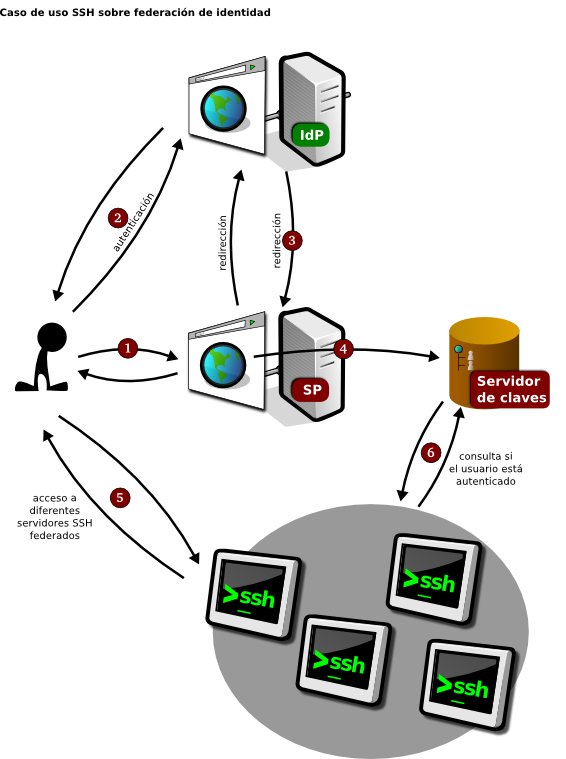
\includegraphics[width=\textwidth]{img/casodeuso1.png}
            \caption{Caso de Uso}
        \label{fig:casodeuso}
    \end{figure}

%TODO importancia del SSH, túneles, importación X

\section{Antecedentes}
    (feide, parche opensshldap)


